\chapter{\normalfont EM TRAINING OF AN INDEL-PHASE PROBABILISTIC MODEL}
\label{ch:indel_phase_model}


\section{Introduction}
Advancement in sequencing technology and bioinformatic tools generate an enormous amount of data from different large-scale projects. The corresponding models and algorithms are also developed to provide solutions to biological and bioinformatic problems. However, probabilistic-based models for indels are far less developed compared with the substitution models. In chapter 3, while I applied a sliding-window method to do the post-aligning indel phase fixation, the proportion of indel phases cannot represent the actual indel rates over the evolutionary time. To solve this, I developed an indel-phase probabilistic model that describes both substitution and indel processes. And I developed a novel EM training method that was capable of estimating the instantaneous indel rates of different phases,  indel length distribution, nucleotide exchangeabilities, non-synonymous selective coefficient, and branch length. The simulation results demonstrated the feasibility and accuracy of our EM algorithm for training the indel-phase model.\\
\indent Many previous papers study the estimation of indel rates and indel length distribution. For instance, \citeauthor{metzler2001assessing} reduced the alignment variability by sampling sequence alignments and estimating the indels from their joint posterior distribution. \citeauthor{holmes2005using} proposed an EM method of estimating the indel parameters derived from the TKF91 model in multiple sequence alignments. \citeauthor{cartwright2009problems} presented an EM algorithm built on a pair hidden Markov model handling indels in neutrally evolving DNA sequences. In those studies, while the indel rates were derived from the observed gap counts between alignments, a single gap actually reflected the possibility of multiple indel events and misled the computation of sequence likelihood. \\
\indent Two main distributions were utilized for describing the indel length: geometric and Zipfian. Although there was evidence that Zipfian distribution fitted better with the biological datasets in both coding \parencite{benner1993empirical} and non-coding regions \parencite{saitou1994evolutionary}, geometric distribution was computationally tractable and easily calculated. Many researches accentuated the difference between insertions and deletions(\cite{tao2007patterns,metzgar2002domain}). They utilized pseudogenes or outgroups to distinguish insertions from deletions, which might increase the memory cost and restrict the data volume. In our research, due to the lack of reference genomes, I presumed one of the two sequences as an ancestor, and the other was automatically assigned as the descendant.\\
\indent The existing methods of training the probabilistic models for indel evolution normally assume a single indel rate for all gaps between sequences, equal length distributions between insertions and deletions; and introduction of alignment bias (\cite{holmes2005using, lunter2007probabilistic, cartwright2009problems}). Here, I introduced several improvements in our indel-phase model study: 1) our indel-phase model proposed three rates of each indel phase instead of one rate for all indel events; 2) this model is richer because of the inclusion of the GTR+MG94 model for describing the substitution process; 3) During the EM training of the indel-phase model, the alignment bias was greatly removed through applying an importance sampling method. 


%%%%%%%%%%%%%%%%%%%%%%%%%%%%%%%%%%%
\section{Methods and Materials} 
\subsection{Indel-phase Model}
I developed an indel-phase model to calculate the likelihood of pairwise alignment, which contained a finite number of states in each indel phase: match($M_i$), insertion($I_i$), deletion($D_i$), waiting($W_i$) (Fig 4.1), where i represented 0,1,2 three phases. This model innovatively splitted the alignment into three independent processes and each of them corresponded to an indel phase, where the insertion, deletion, and substitution process should occur. Hence, this model required each codon as a unit. The circle represented a single state, and the arrows connecting each state carried a transitional probability weight. Of note, the waiting state served to simplify the transitional probability calculation without actual evolutionary meaning. Our alignment was normalized so that the insertions always occurred before deletions within the same indel phase. The N:N edge emitted a codon substitution matrix as the emission weights. The 0:N edge emitted inserted codons and N:0 edge deleted codons from the alignments.   
\newpage
\begin{figure}[H]
     \centering
     \begin{minipage}[t]{1\textwidth}
     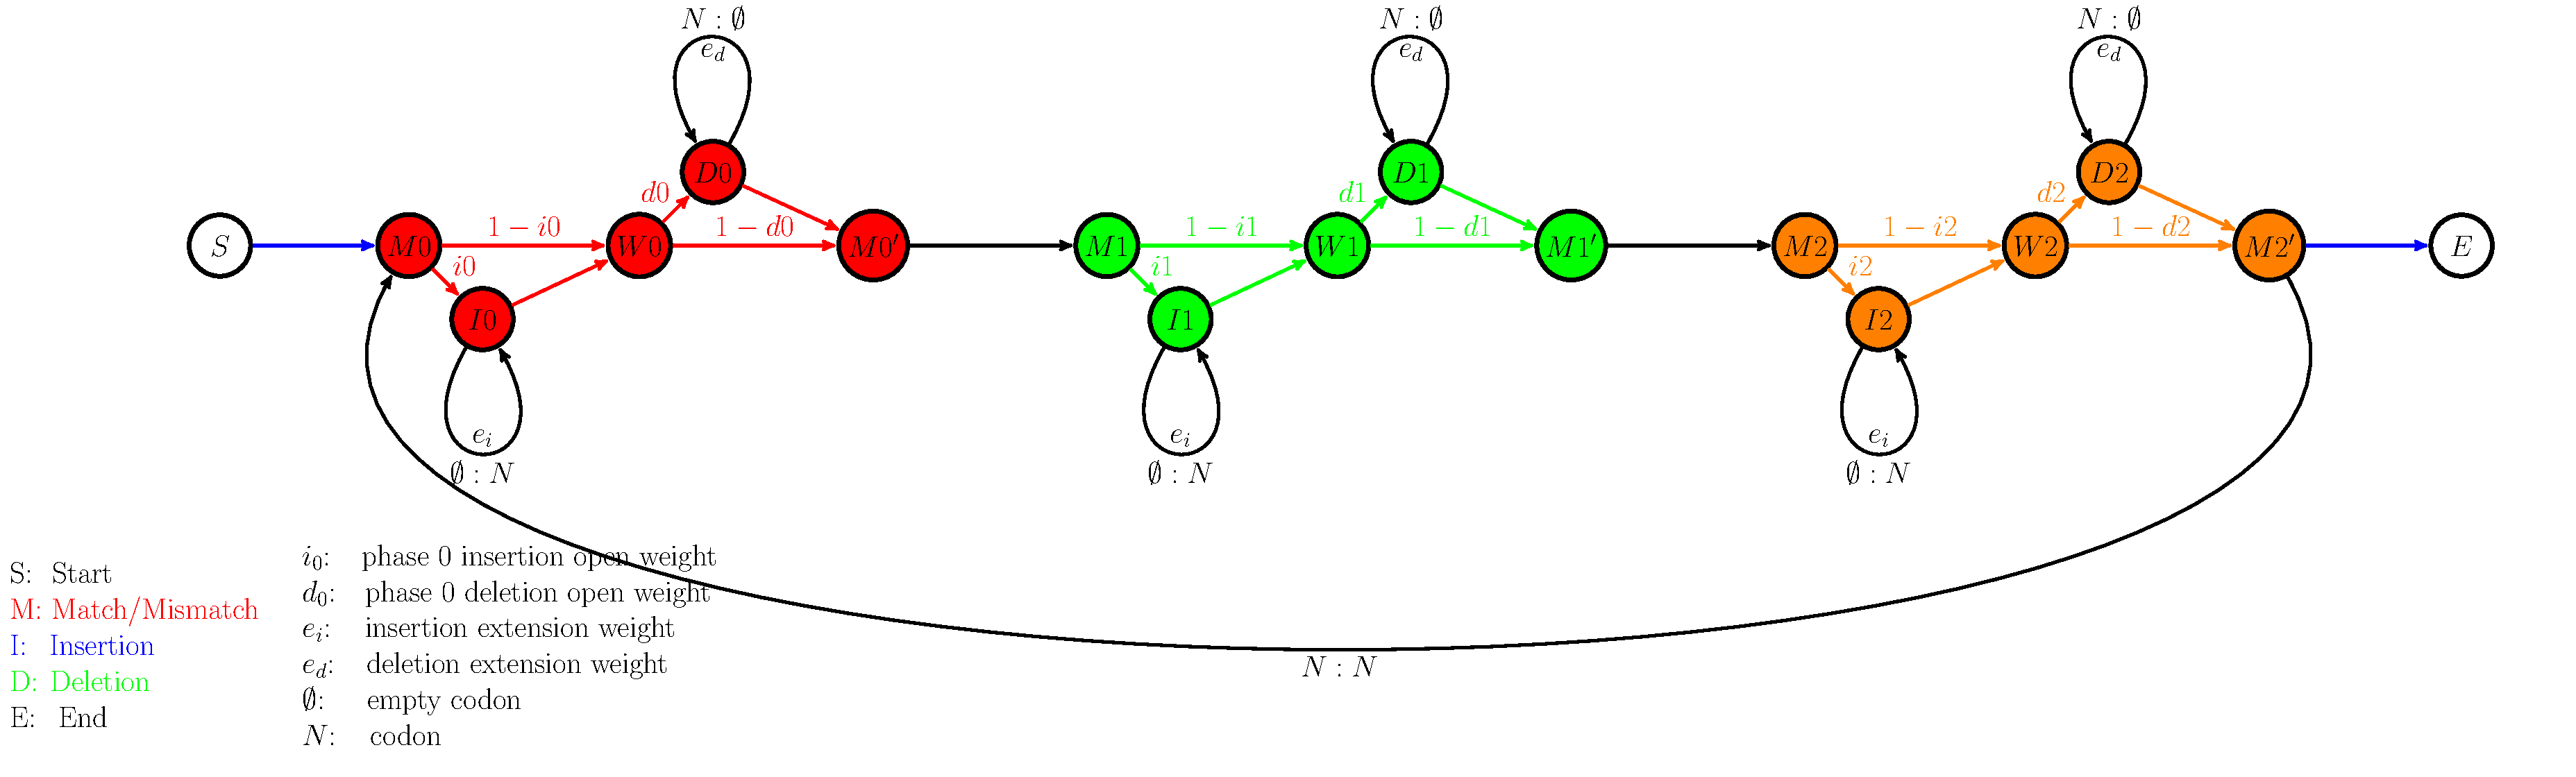
\includegraphics[width=\linewidth,height=5cm]{Fig1.pdf}
     \titlecaption{Indel-Phase Probabilistic Model}
     { {Transition probabilities are shown above each arrow. The model contains start(S), match(M), insertion(I), deletion(D), waiting(W), and end(E) states. Note that the waiting, start, and end states are considered as null state.} 
     \par}
     \end{minipage}
\end{figure}

\subsection{Indel Rates}
Abstractly, we treat gaps as one or more overlapping or neighboring indels assembling together, whereas an indel is a specific evolutionary event that adds or deletes residues from a sequence. Without ancestor lineage reference, a gap in the alignment of one sequence may be caused by either one or more deletions in that sequence or one or more insertions in the other sequence. Popular methods like maximum parsimony tend to reassemble adjoining single indel events so that the alignment scores can be maximized, which underestimates the true indel rate along an evolutionary branch \citeauthor{knudsen2003sequence}. To simplify the model, I treat a single gap from the alignments as a single indel event. Next, the model assumes both substitutions and indels follow a continuous-time Poisson process. If the chain does not terminate, the probability of the next state of I or D is $g_i = 1-e^{r_i t}$, where $r_i$ is the instantaneous indel rate of phase i relative to substitution rate, t is the branch length between pairwise sequences measured in expected number of  substitutions per base pair. SO the $e^{r_i t}$ represents the probability that no indel events have occurred.

\subsection{Indel Length Distribution}
I assumed the length of insertions and deletions followed different geometric distributions in our model. The maximum likelihood estimate of gap extension weight $e_i, e_d$ is calculated by $ 1-1/\hat{g_s}$, where $\hat{g_s}$ represented the average gap size of insertions and deletions separately (dividing the sum of gap length by the total number of gaps).   

\subsection{Codon Substitution Model}
The substitution matrix $R_{ij}$ was represented by the MG94 +GTR codon substitution model (\cite{muse1994likelihood, tavare1986some}), and the details about the matrix construction can be found in the methods of chapter 2. 

\subsection{Coati-sampling Method}
To fulfill the purpose of aligning coding sequences as codons but also allows indels within codons, I select the Coati-sampling aligner that is built on the Forward algorithm within the context of Hidden Markov model developed by our lab (\href{https://github.com/jgarciamesa/coati}{https://github.com/jgarciamesa/coati}). This aligner has no restrictions for gap locations, options for forcing the gap length to be multiple of three nucleotides, and more importantly, allows to generate many sample alignments for a single pairwise sequence with a sequence likelihood.  

\subsection{EM Method}
I used the EM method to find the local maximum likelihood estimates of parameters. The E-step generated a function for the expectation of the log-likelihood: 
\begin{gather*} 
\begin{aligned}
 Q(\theta|\theta_{t}) 
 &= \sum_{i}\sum_{j} D_{ij}log(P_{ij})\\
 &+ N_0log(g_0) + M_0log(1-g_0) + N_1log(g_1) + M_1log(1-g_1) + N_2log(g_2) + M_2log(1-g_2) \\
 &+ (L_i - N_i)log(e_i) + N_{i}log(1-e_i) +  (L_d - N_d)log(e_d) + N_{d}log(1-e_d)\\
 &- \sum_{1}^n log(\Pi_{k}) - \sum_{1}^m log(\Pi_{k})
\end{aligned}
\end{gather*}
\\
\noindent where $D_{ij}$ is the codon substitutions $i \rightarrow j$ observed from data, $P_{i,j}$ is the codon substitution matrix from i to j ($1 <= j <= 64$), which is calculated as the exponential of the rate matrix $R_{ij}$. $N_0$, $N_1$, $N_2$ is the total number of gaps phase0, phase1, and phase2, $g_0$, $g_1$, $g_2$ is the gap openings of three phases. $M_0$, $M_1$, $M_2$ is the total number of non-gap phases, which equals the difference between codon lengths and number of gap phases. $L_i$, $L_d$ are the total length of inserting gaps and deleting gaps, $N_i$, $N_d$ are the total number of inserting gaps and deleting gaps, $e_i$, $e_d$ is the gap extensions of insertion and deletion events. $\pi_k$ represents the nucleotide frequency of ancestor and descendent sequences in which the lengths are n and m. I removed their likelihood because they stayed invariant in all of the aligning samples. In addition, the E-step has a time complexity of number of sequences times sequence length O(500*100). Hence, I developed a grouping method within the E step to speed up the performance: 1) Dividing the groups to ensure that each group has identical alignments. 2) recording the likelihood of each group alignment; 3) extracting the number of groups and group size. \\
\indent The M-step maximizes that function with respect to the parameters $\theta$ via utilizing the summary statistics obtained from E-step. 
\begin{gather*}
              \theta_{t+1} = \underset{\theta}{argmax}Q(\theta |\theta_{t})
\end{gather*}
Where $\theta$ represents our parameter set \{$6\sigma s, \omega,\tau, g_i,e_i$\}. Gap opening weight $g_i$ and gap extension weight $e$ was solved by taking the first derivative of likelihood function Q and the value was $N_i/(N_i+M_i)$ and $1-1/(L/N)$ respectively. For practical purposes, I utilized the Nmkb derivative-free optimization method to obtain the estimates of substitution models within M-step. Finally, I used the root mean square error ($<10^{-4}$) between the joint estimates and true parameters as the stop criterion for the EM process.    

\subsection{Importance Sampling}
Doing the sum over all possible alignments for the indel-phase model is expensive due to the indels happening inside codons. Instead I utilized COATi to sample alignments and applied an importance sampling method to estimate the required statistics for the EM. Importance sampling is a statistical technique that is used to estimate the properties of a particular distribution without sampling from that distribution directly. \parencite{kloek1978bayesian}. In our research, two distinctive distributions are from the indel-phase model and coatiM model respectively. The indel-phase model is capable of calculating the likelihood of the alignment without actually generating the alignment samples. For example, I was able to obtain 100 samples from each unaligned pairwise sequence after the coati alignments, and calculated their sequence likelihood g(x). Then I generated a second likelihood value f(x) of the same alignments from our indel-phase model. The likelihood ratio of f(x)/g(x) is called the importance weight w, which is the key for correcting the distribution difference between two models. Because it always encourages a higher weight to frequently occurring aligning samples. For example, for a 100 alignment samples $A_i$, the average weighted number of gaps  is $\hat N$=$\sum_{i}^n w_i N(A_i) /100$. Additionally, for the convenience of calculation, we used the normalized importance weight instead of the raw weight, because sometimes I can only compute w up to a proportionality constant. 

\subsection{Parameter Space}
I need to assign an appropriate weight space for our true parameters $\{\pi, \sigma, \tau, \omega, g_i, e\}$.1) The four nucleotide frequencies $\pi$, six nucleotide exchangeabilities $\sigma$ , and selective strength on non-synonymous substitutions $\omega$, are generated via the same methods of chapter 2. This time I selected a smaller $\tau$ value to avoid the possibility of overlapping indels. 2) The gap opening weight are represented by the formula $1-e^{r t}$ with indel rate r, in which the indel rate is about 12-16 indels per 100 substitutions according to \citeauthor{cartwright2009problems}. And the indel rates of three phases are mutually independent and within the range \{0.05,0.15\} when the substitution rate is normalized as 1. 3) The gap extensions are represented by the average gap size of $1-1/g_s$, where $g_s$ is determined in the unit of codons instead of nucleotides. I selected a boundary of gap size \{1,4\}, ensuring that the gap extension weights were always positive, and the largest gap was the same as the size used in the sliding window method of chapter 3.  

\subsection{Gillespie Simulation}
I need to simulate a series of true alignment based on my generated true parameters. \citeauthor{gillespie1977exact} proposed an algorithm that was able to generate a statistically correct trajectory of a stochastic equation system, which has been applied on simulating the evolutionary process of a single DNA sequence \parencite{sipos2011phylosim}. The probability of a random event occurring equals the $r_i/(\sum_{i=1}^n r_i)$. Our gillespie algorithm separates all three processes (deletion, substitution, insertion) to make it easier to estimate parameters. Without separation there would be ambiguity when multiple events happen at one codon. \\
\indent There are several key points about our gillespie algorithm: 1) since both mutations and indels follow a continuous-time Poisson distribution, I must use the same branch length $\tau$ for all three independent processes (deletion, substitution, and insertion). 2) Different indel phases can occur at different rates r0, r1, r2. 3) The indel lengths are a multiple of three nucleotides and follow a geometric distribution. Inserted nucleotides are drawn from the stationary distribution of nucleotide frequencies. 4) No substitutions will occur inside the inserted fragments. 5) The total number of inserting positions is n+1, if the sequence length were n. The first inserting position is on the left side of the first nucleotide, which is normally called the immortal link. The total number of deleting positions equals the sequence length n \parencite{thorne1991evolutionary}. 6) Alignments are normalized such that insertions occur before deletions of the same indel phase. 7) The evolutionary order of our Gillespie simulation is deletion $\rightarrow$ substitution $\rightarrow$ insertion, because this is a symmetric model for calculating likelihood. It guarantees that the evolutionary track of a substitution process never gets wiped out because the mutational type (synonymous or nonsynonymous) of a codon surrounding an indel stays unchanged after the alignment. 8) The waiting time between each evolutionary event follows an exponential distribution, and the simulation process stops until the accumulated time passes our branch length $\tau$. 

   


%%%%%%%%%%%%%%%%%%%%%%%%%%%%
\section{Results}
\subsection{Gillespie Simulation Results}
To establish a baseline for the performance of our method, we generated a qqplot for each parameter. Figure 4.2 displays the correlation between the true parameters and parameter estimates from gillespie simulated alignments. The diagonal line measures the accuracy between the true and estimated parameters. Since the Gillespie simulation only generates the true alignment, their differences are due to the randomness of the simulation process instead of any systematic error. 
\begin{figure}[H]
     \centering
     \begin{minipage}[t]{1\textwidth}
     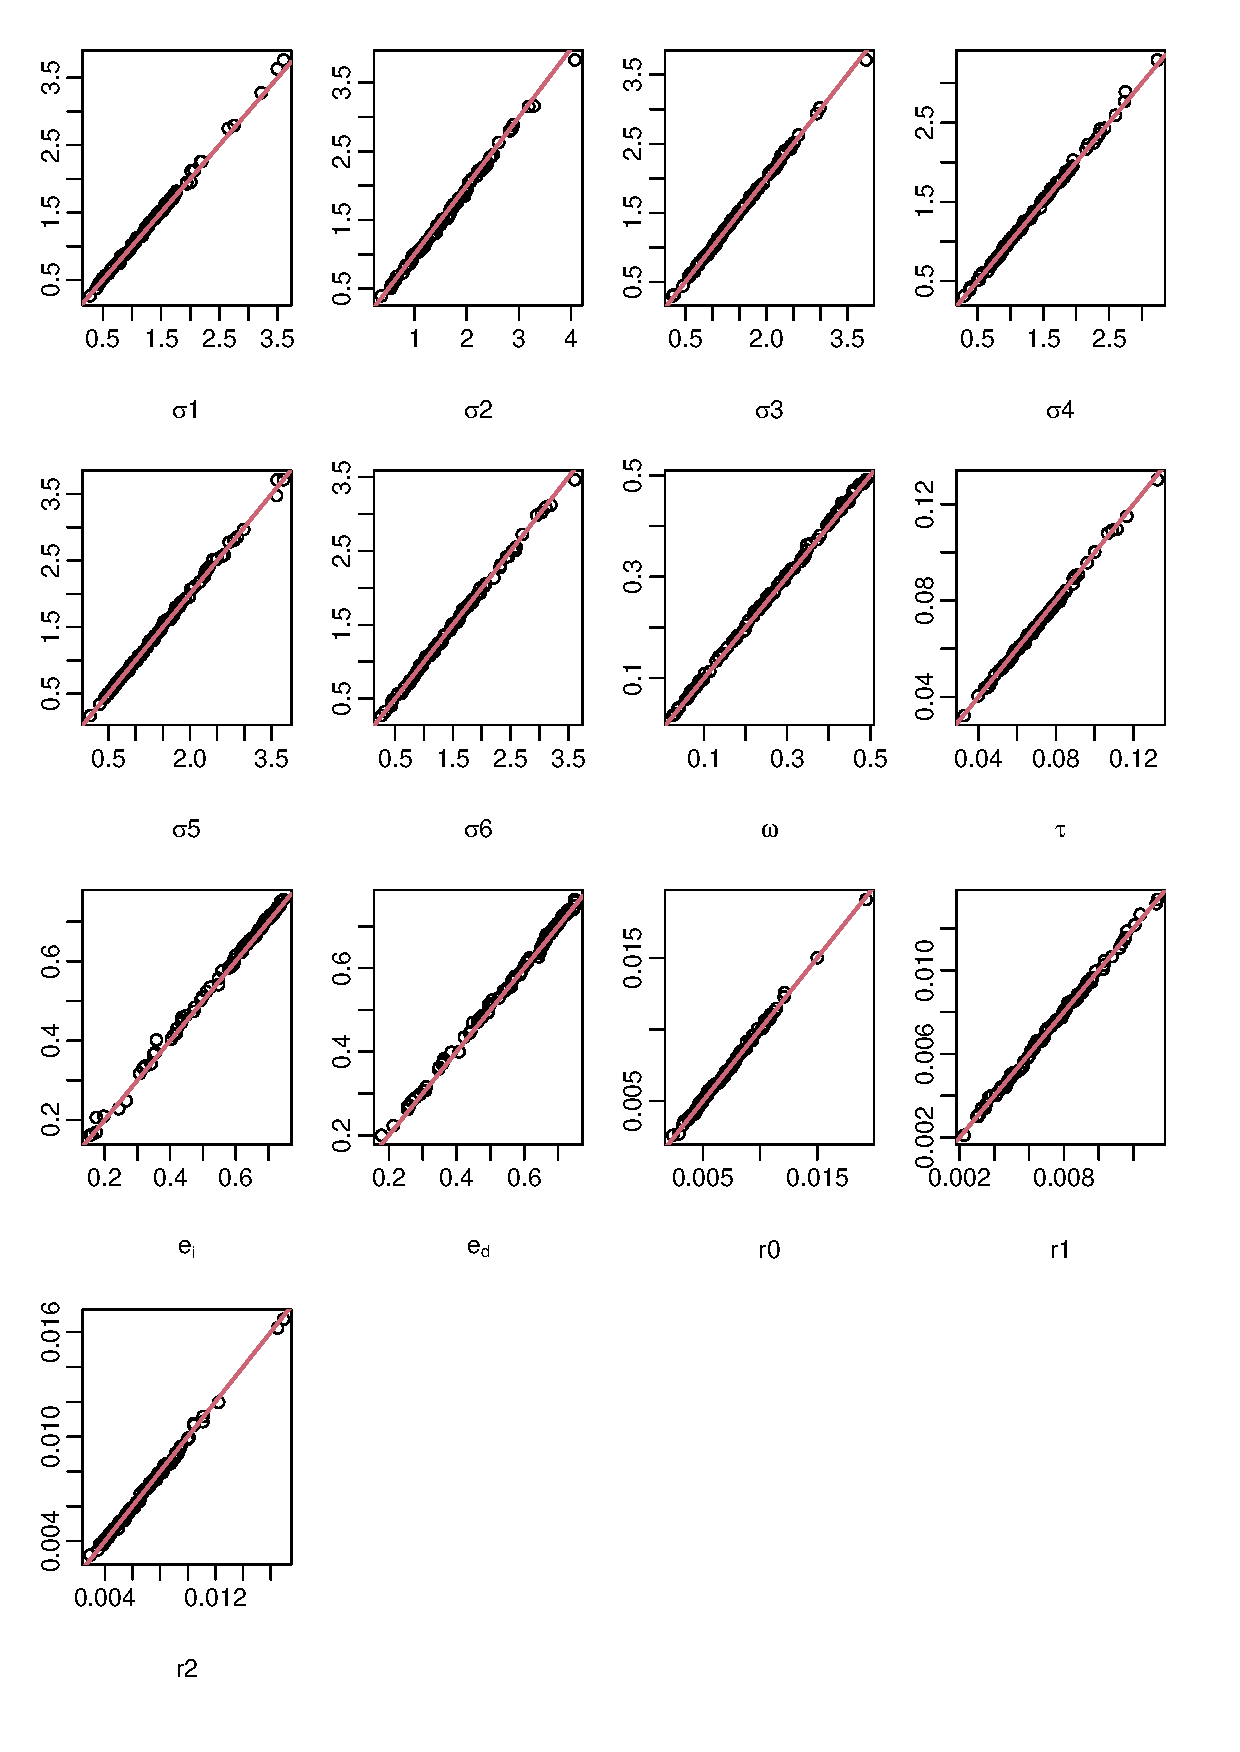
\includegraphics[width=1\linewidth,height=1.2\linewidth]{Fig2.pdf}
     \titlecaption{QQplot of 13 Parameters via Gillespie Simulation.}
     { {True parameter values are on the x-axis and parameter estimates are on the y-axis, including Six $\sigma$s, $\tau$, $\omega$, gap extensions $e_i$, $e_d$, and three indel phase rates $r0$, $r1$, $r2$.}
 \par}
     \end{minipage}
\end{figure}
\newpage
\indent Figure 4.3 displays the distribution of error percentage between the true and estimated parameters across 100 simulations. I measured the error percentage as an absolute value of (true-est)/true and was always positive. The mean value of error percentage is extremely low as well as the variance. For example, the lowest and highest mean value of  error percentage is 0.013 ($\tau$), and 0.027 ($r_0$) (table \ref{tab:error_stat1_cha3}).
\begin{figure}[H]
     \centering
     \begin{minipage}[t]{1\textwidth}
     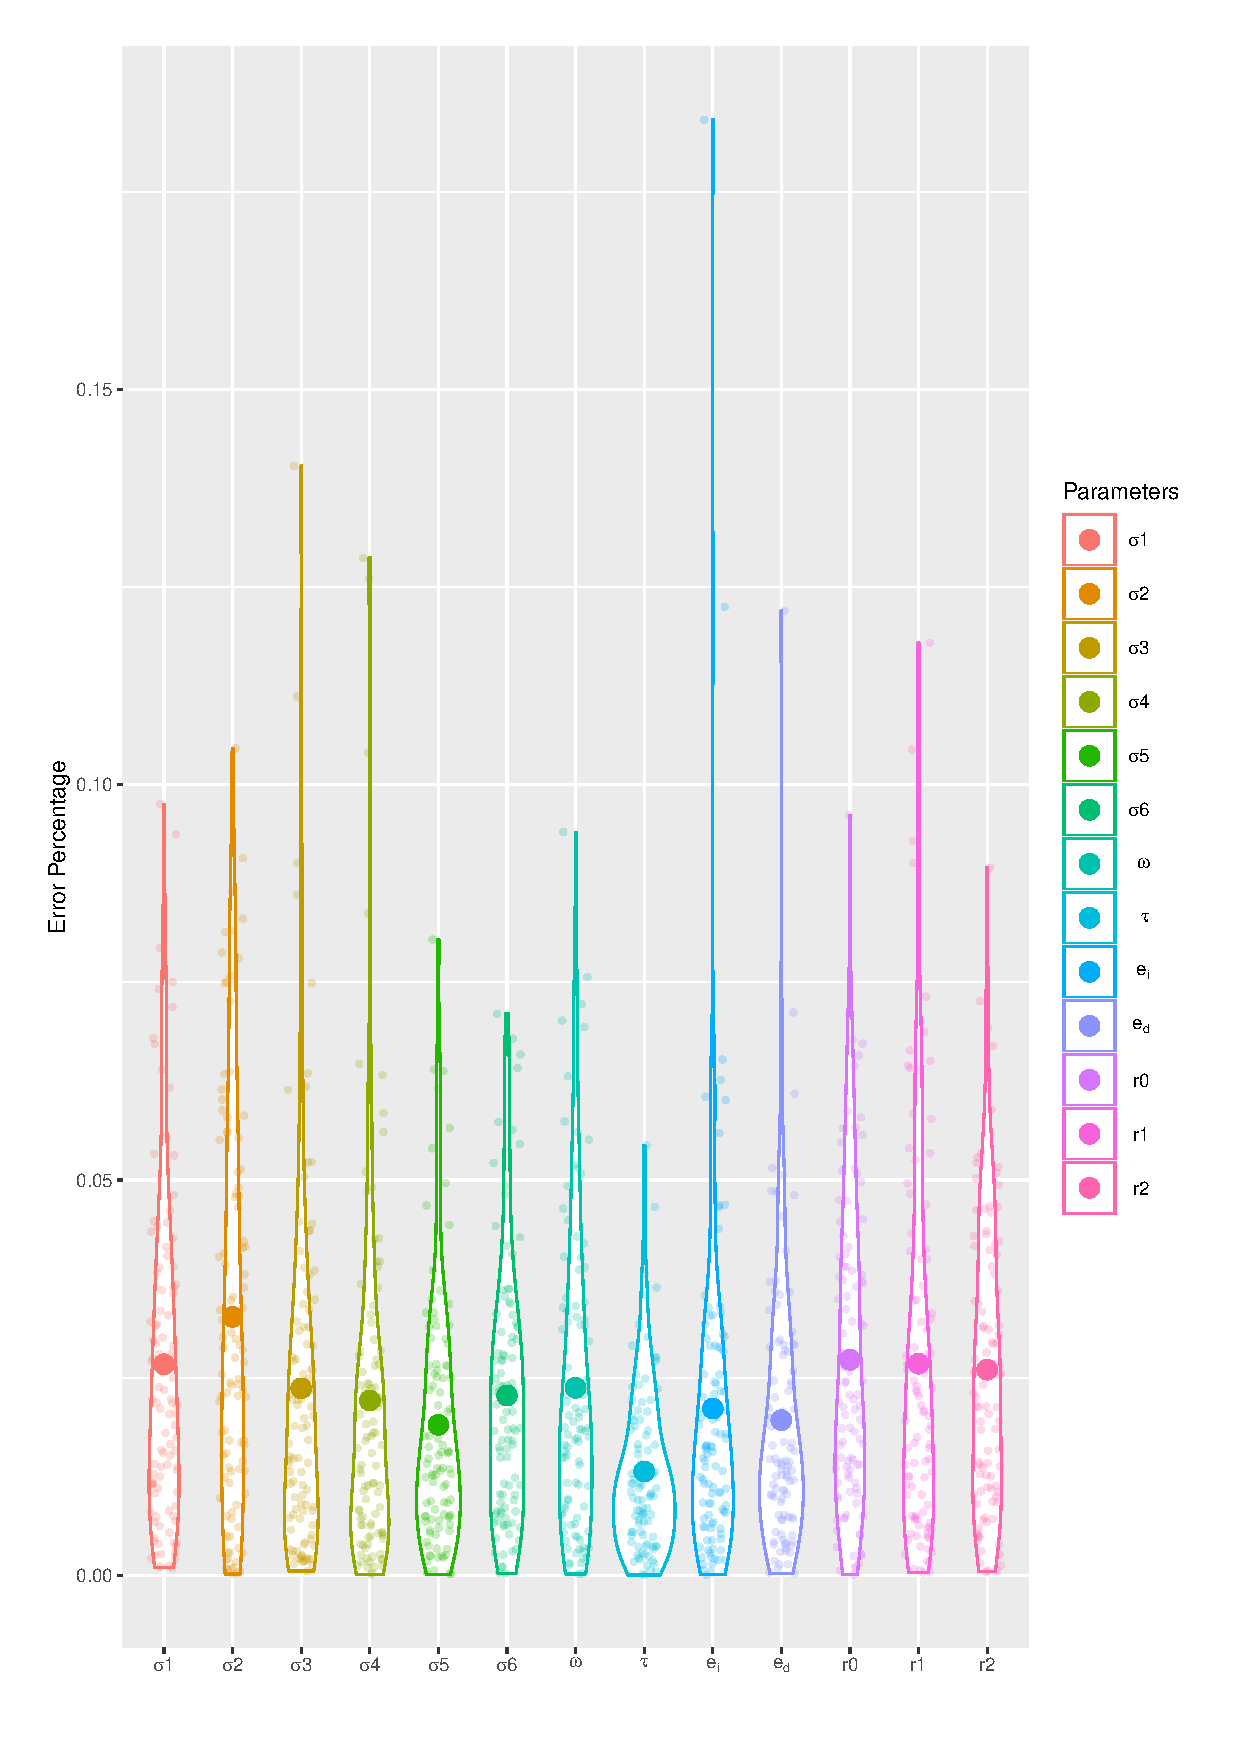
\includegraphics[width=1\linewidth,height=1\linewidth]{Fig3.pdf}
     \titlecaption{Error Percentage Distribution Plot of 13 Parameters via Gillespie Simulation.}
     { {Each color represents a parameter estimate.} 
 \par}
     \end{minipage}
\end{figure}

\newpage
\begin{xltabular}{\textwidth}{X| X X X X X X X X X X X X X}
\toprule
& $\sigma_{AC}$ & $\sigma_{AG}$ & $\sigma_{AT}$ & $\sigma_{CG}$ & $\sigma_{CT}$ & $\sigma_{GT}$ & $\omega$ & $\tau$ & $e_i$ & $e_d$ & r0 & r1 & r2 \\
\midrule
\csvreader[]{cha3/table/error_stat1.csv}{}
{\\ \csvcoli & \csvcolii &\csvcoliii &\csvcoliv &\csvcolv &\csvcolvi &\csvcolvii &\csvcolviii
&\csvcolix &\csvcolx &\csvcolxi &\csvcolxii &\csvcolxiii &\csvcolxiv}
\\ \bottomrule
\titlecaption{The Mean and Variance Table of Error Percentage of Parameters from Gillespie Simulation}{$\mu$ and s represent the mean and variance value.}
\end{xltabular}
\label{tab:error_stat1_cha3}

\subsection{EM + Importance Sampling Results}
To examine the performance of our importance sampling method and the EM algorithm, I generated a qqplot for each parameter. Figure 4.4 displays the correlation between the true parameters and our parameters estimates . Almost every simulated point remains on the diagonal line. Since the importance sampling and EM method works on a series of unaligned sequences, the error percentage is considered as the combination of the randomness from Gillespie simulation and the sampling noise from our method. Theoretically, the more samples generated, the more accurate the parameter estimates are.   
\begin{figure}[H]
     \centering
     \begin{minipage}[t]{1\textwidth}
     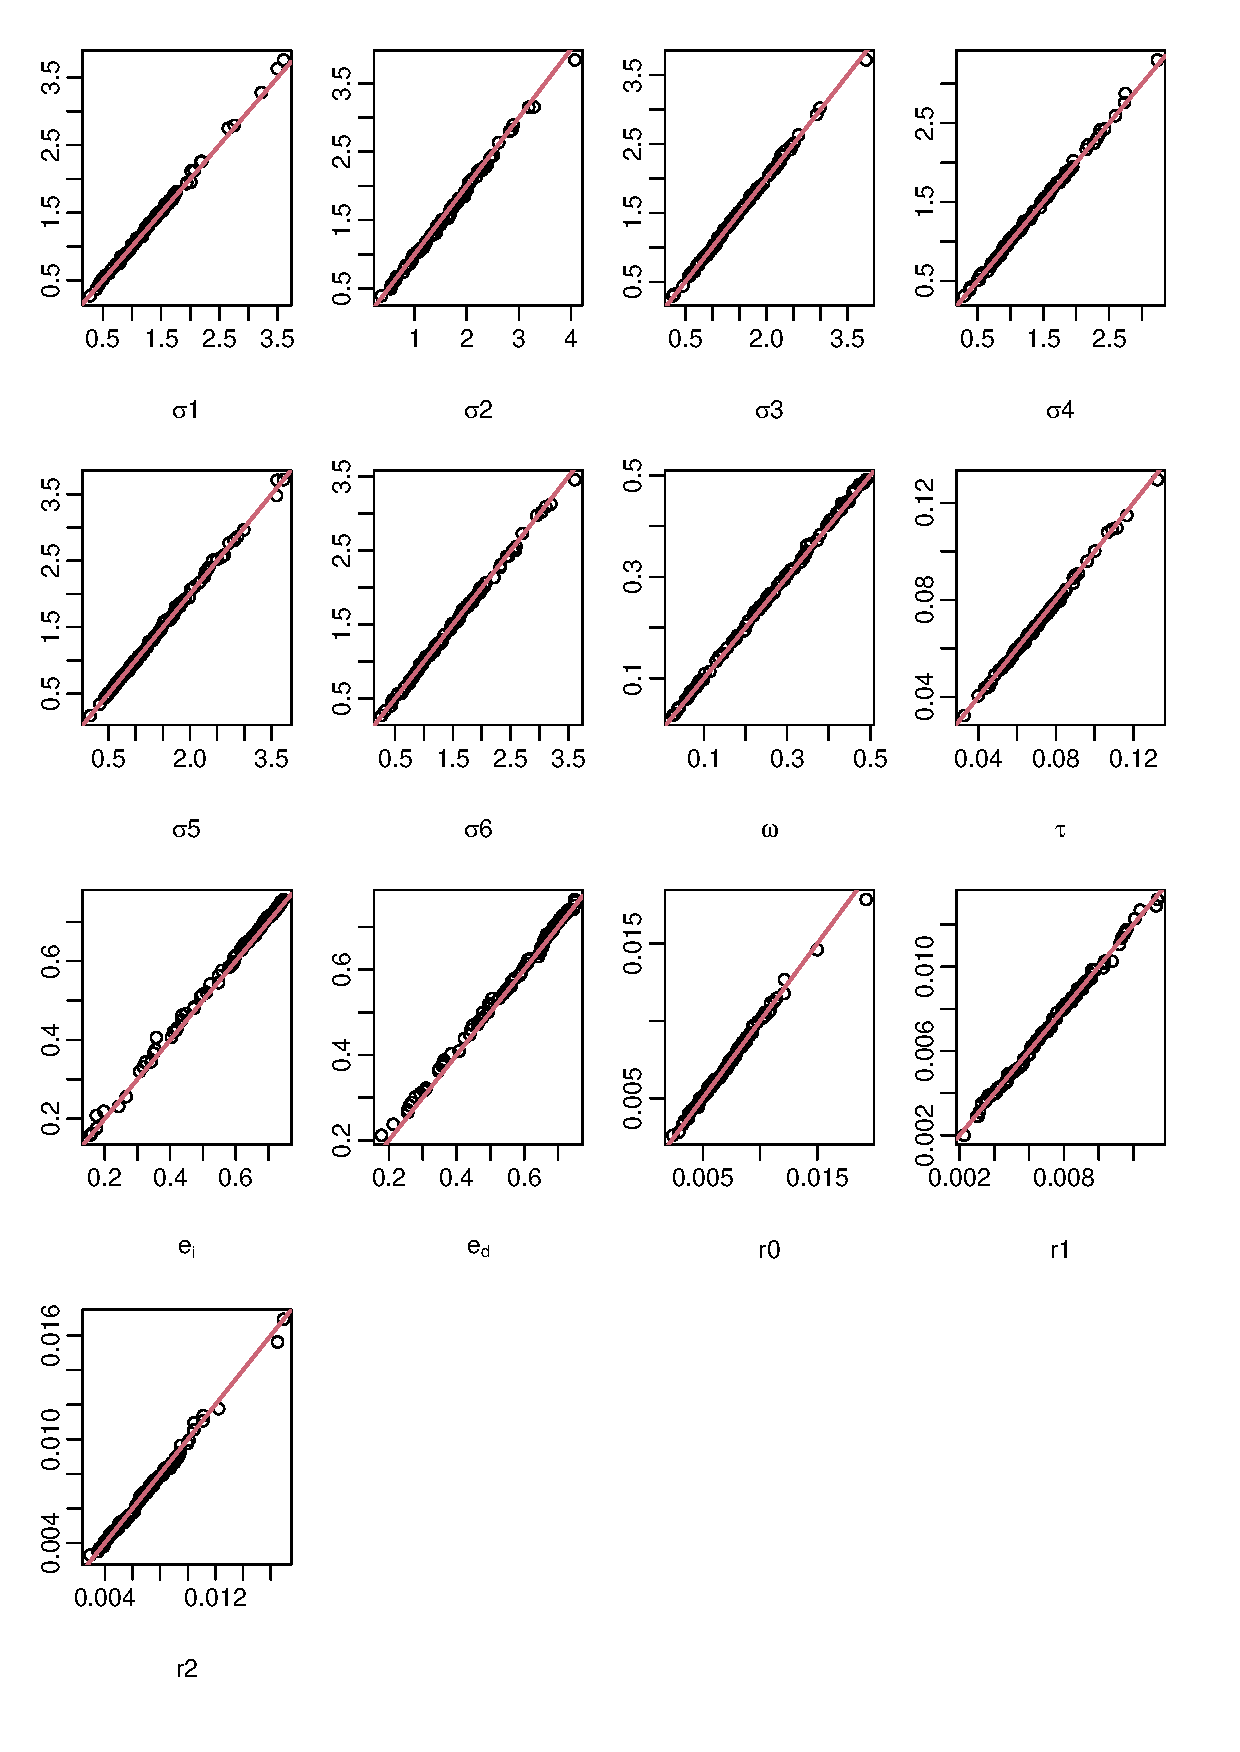
\includegraphics[width=1\linewidth,height=1.2\linewidth]{Fig4.pdf}
     \titlecaption{QQplot of 13 Parameter Estimates via EM + Importance Sampling Method.}
     { {True parameter values are on the x-axis and parameter estimates are on the y-axis, including Six $\sigma$s, $\tau$, $\omega$, gap extensions $e_i$, $e_d$, and three indel phase rates $r0$, $r1$, $r2$.} 
 \par}
     \end{minipage}
\end{figure}

\newpage
\indent Figure 4.5 displays the distribution of error percentage between the true and estimated parameters across 100 simulations. Similarly, the mean value and variance of error percentage for each parameter are extremely low. For instance, the range of the average error percentage value of 13 parameters is [0.013, 0.036] from $\tau$ and $r_0$ respectively (table \ref{tab:error_stat2_cha3}. 
\begin{figure}[H]
     \centering
     \begin{minipage}[t]{1\textwidth}
     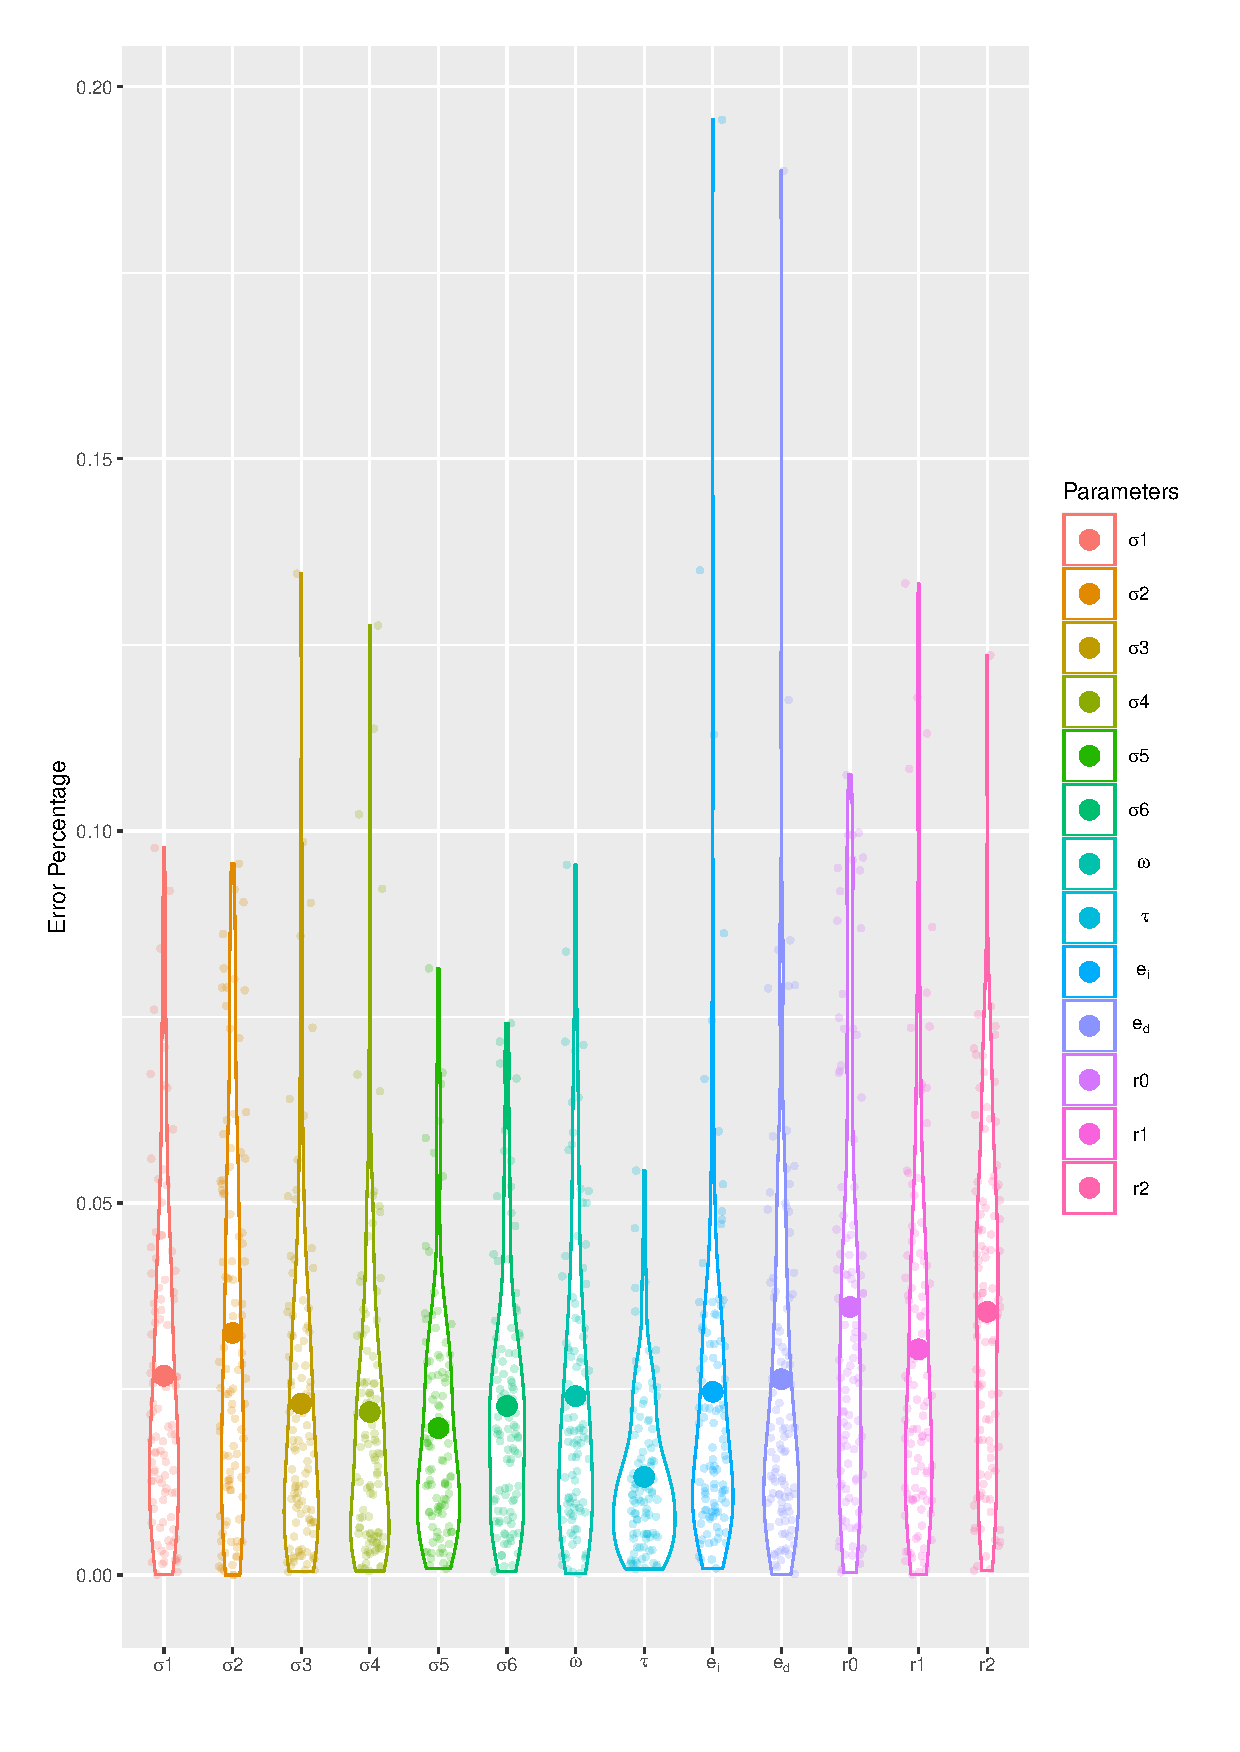
\includegraphics[width=1\linewidth,height=1\linewidth]{Fig5.pdf}
     \titlecaption{Error Percentage Distribution Plot of 13 Parameters via EM + Importance Sampling Method.}
     { {Each color represents a parameter estimate.} 
 \par}
     \end{minipage}
\end{figure}

\newpage
\begin{xltabular}{\textwidth}{X| X X X X X X X X X X X X X}
\toprule
& $\sigma_{AC}$ & $\sigma_{AG}$ & $\sigma_{AT}$ & $\sigma_{CG}$ & $\sigma_{CT}$ & $\sigma_{GT}$ & $\omega$ & $\tau$ & $e_i$ & $e_d$ & r0 & r1 & r2 \\
\midrule
\csvreader[]{cha3/table/error_stat2.csv}{}
{\\ \csvcoli & \csvcolii &\csvcoliii &\csvcoliv &\csvcolv &\csvcolvi &\csvcolvii &\csvcolviii
&\csvcolix &\csvcolx &\csvcolxi &\csvcolxii &\csvcolxiii &\csvcolxiv}
\\ \bottomrule
\titlecaption{The Mean and Variance Table of Error Percentage of Parameters from EM + Importance Sampling Method}{$\mu$ and s represent the mean and variance value.}
\end{xltabular}
\label{tab:error_stat2_cha3}

\section{Discussion}
To understand the evolutionary process of substitution and indels together, I first utilized the Gillespie simulation to generate a series of true alignments. Due to the complexity of the model, I developed an EM + importance sampling method to train the indel-phase model with unaligned sequences (removing the gaps from the Gillespie simulated alignments), and measured the accuracy of the parameter estimates. By marginalizing over all sampling alignments, I was able to obtain the accurate parameter estimates by greatly removing the alignment bias and reducing the sampling variance through a large sample size.  \\ 
\indent It is worthy of pointing out that the parameter that has the lowest average value of error percentage is  $\tau$, and the highest one is $r_0$  in both Gillespie simulation and EM + importance sampling process. It is well known that the substitution events occur much more frequently than the indels during the same evolutionary time (branch length). And the branch length $\tau$ actually measures the number of substitutions per site that is expected to be much higher than the number of indels per site. Similarly, the general error percentage of substitution-relevant parameters \{$6\sigma s, \omega, \tau $\} are lower than the indel-related parameters \{$r_0, r_1, r_2,  e_i, e_d $\} during the same evolutionary time. \\
\indent In the future, I am able to vary our indel-phase model to get better performance. For example, I can utilize the zeta distribution instead of the traditional geometric distribution for indel length since \citeauthor{cartwright2009problems} mentioned the zeta power-law model might be a better fit based on many empirical studies. Additionally, I can convert our R scripts to C++ and improve the computational speed for the EM training process, allowing us to increase the sample sizes to obtain more accurate parameter estimates.   







%\bibliographystyle{unsrtnat}
%\bibliography{ref3.bib}


